\chapter{Data Understanding}

\section{Initial Data Collection}

\paragraph{Data Requirements Planning}
The business objective is the development of a solution for the automatic aggregation of documents based on their topics. To achieve this goal, a sufficient number of documents are required. Also, the documents must contain enough text to be assigned a topic. After clustering the value of each expense in a cluster have to be summed, to gain the desired insight of spending in one category. So the value an expense amounts to has to be included in the data.

\paragraph{Selection Criteria}
An initial look a the data has shown that each invoice item can easily contain more than 100 pieces of information, which can be considered as attributed in the dataset. The part of the data that is of interest for the research is the description and payment data. Other data needs to be retained for a coherent and informative presentation of the results, such as location information and information on seller and buyer.

\paragraph{Insertion of Data}
The insertion of data is concerned with the theoretical utilization of the data and problems arising during this process. The encoding and grouping of free text items is referenced as one concern in the \ac{CRISP-DM} user guide \cite[p.~44]{CRISPDM2000}. In this research the focus is on free text items, therefore this step will be discussed in detail in the following chapter. 
Other concerns are missing attributes. The dataset has already undergone a surface-level evaluation, which concludes that all relevant attributes are contained.

\section{Data Description}
The data is available as 152,591 \ac{JSON} files. Each file represents one invoice document. 

Each invoice contains specific header data, the detailed list of the 172 header fields is contained in the appendix (\ref{invoice-header}). 
The items listed in one invoice are line items. The information about line items is contained in 32 features, also detailed in the appendix (\ref{invoice-lines}).

All documents follow a specific schema (\ref{code:JSONSchema}). In the beginning, the metadata of the invoice is described, followed by an array of objects (l.7). Each item in the array contains two key value pairs. First, the label of the feature (e.g. "totalAmount"). Second, the value of the feature (e.g. "\$7").


\lstinputlisting[
label=code:JSONSchema,    % Label; genutzt für Referenzen auf dieses Code-Beispiel
caption=Shortened JSON Schema of one invoice document representation,
captionpos=b,               % Position, an der die Caption angezeigt wird t(op) oder b(ottom)
style=EigenerPythonStyle,   % Eigener Style der vor dem Dokument festgelegt wurde
firstline=0,                % Zeilennummer im Dokument welche als erste angezeigt wird
lastline=23                 % Letzte Zeile welche ins LaTeX Dokument übernommen wird
]{Quellcode/json-schema.json}



\section{Data Exploration}
The exploration focuses on the descriptions and related metadata, as only this part of the data is used for modeling.
\paragraph{Descriptions}
The descriptions of invoice items vary greatly in their length. While the largest portion of descriptions is under 600 characters, there are outliers with over 1000 characters. 
\begin{figure}[h!]
	\centering
	\includegraphics[height=6cm]{Bilder/hist_description.pdf}
	\caption{Histogram of Description Length}
	\label{fig:descr-length}
\end{figure}

\begin{figure}[!h]
	\centering
	\includegraphics[height=8cm]{Bilder/data_understanding/toptendescr.png}
	\caption{Top ten most frequent descriptions}
	\label{fig:descr-most-frequent}
\end{figure}
The top ten most frequent descriptions are led by two values which will be removed during data cleaning. The first value ('nan') is short for 'not a number'. The second most frequent description is an empty value. Unfortunately, these descriptions amount for one fourth of all text elements. The next descriptions are more speaking, for example consulting fees, credit card transaction fees, and payments for room and board.

\begin{figure}[!h]
	\centering
	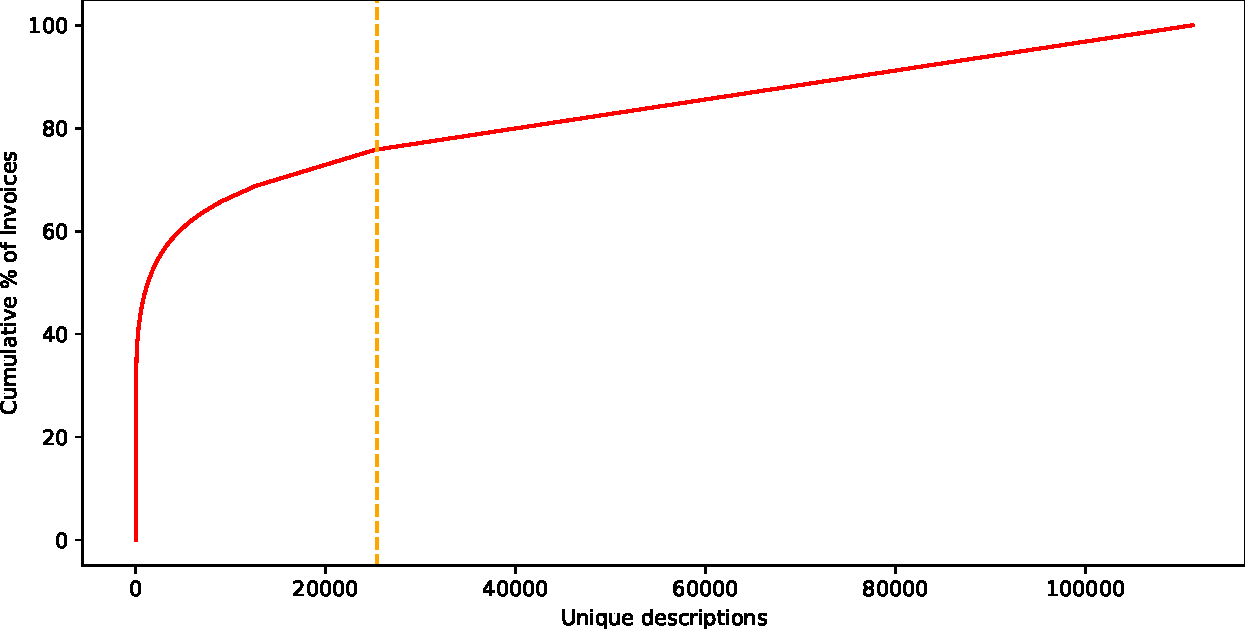
\includegraphics[height=6cm]{Bilder/data_understanding/descriptions_pareto.pdf}
	\caption{Percentage of Invoices by cumulative unique Descriptions}
	\label{fig:descr-hist}
\end{figure}
The frequency distribution of unique descriptions shows that the top third (36\%) of the descriptions covers 80\% of the invoices. It is notable, that the slope shows an edge at the point of the 24212the description. After this point, each following description only occurs once in the whole dataset. In turn, this means that only 20\% of the descriptions occur more than once.
\paragraph{Language Distribution}
The description of the invoices is related to the feature 'language', which describes the language of the invoice and its text fields. The most popular languages are English, Spanish, and German. It is noticeable, that there are over 700 languages or combinations of more than one language. 58878 invoices were not assigned a language, which is roughly one third of the total number.
\begin{figure}[h!]
	\centering
	\includegraphics[height=6.5cm]{Bilder/languages.pdf}
	\caption{Number of Invoices per Language}
	\label{fig:languages-bar}
\end{figure}

\begin{figure}[h!]
	\centering
	\includegraphics[height=6.5cm]{Bilder/languages_pareto.pdf}
	\caption{Percentage of Invoices by cumulative Number of Languages}
	\label{fig:languages-pareto}
\end{figure}


From the chart (\ref{fig:languages-pareto}) it can be inferred, that 80\% of invoices are in the top 16 languages. The slow rise after the top 80 languages indicates, that there are a lot of languages with a small number of invoices. This is also explained with a huge number of possible combinations of more than one language.


\paragraph{Invoice Item total Amount}
The invoice item total amount stands for the charge corresponding to one line in an invoice. Without very basic data cleaning, this column was not usable. The values were separated by a variety of different decimal delimiters and contained additional symbols. Also, the variation was initially very high due to some outliers in the magnitudes of $10^{217}$. Therefore, the values were aligned to one common decimal delimiter and stripped of the 1st and 99th percentile. This allows an initial insight into the distribution of the values.

\begin{table}[!h]
	\caption{Five-number summary for Item total Amounts}
	\centering
	\begin{tabular}{llllllll}
		\toprule
		 \textbf{mean} & \textbf{std. dev.} & \textbf{min} & \textbf{25\%} & \textbf{50\%} & \textbf{75\%} & \textbf{max} \\
		\midrule
		  4,749.69      & 17,687.85          & 1.64         & 45.84         & 276.20        & 1,520.00      & 197,721.71  \\
		\bottomrule
	\end{tabular}
\end{table}

The five-number summary shows that the values are skewed to the right in a considerable manner. The so-called tail of the price distribution reaches almost the 200,000 mark. For the further analysis, it will be interesting if very large charges belong into a similar group of spending.

\section{Data Quality}
In the analyses before several problems with the data could already be identified. Firstly, a lot of descriptions are empty or have the unusable value 'nan'. Secondly, the language distribution has shown that the spread is highly biased towards English. 
Both the unusable values and the uneven language distribution will be addressed in the data cleaning part of the thesis.

The quality of data for text mining purposes can be evaluated using four elementary dimensions \cite[p.~1279]{dataQualityAzeroual} :

\begin{table}[!h]
	\begin{tabular}{lll}
		\vspace{0.5cm}
		\textbf{Completeness}                                                        & \begin{tabular}[c]{@{}l@{}}The extent to which data are of sufficient breadth, depth, \\ and scope for the task at hand\end{tabular}              &  \\
		\vspace{0.5cm}
		\textbf{Correctness} & The extent to which data is correct and reliable                                                                                                  &  \\
		\vspace{0.5cm}
		\textbf{Timeliness}                                                          & \begin{tabular}[c]{@{}l@{}}The extent to which the age of the data is appropriate \\ for the task at hand\end{tabular}                            &  \\
		\vspace{0.5cm}
		\textbf{Consistency}                                                         & \begin{tabular}[c]{@{}l@{}}The extent to which data are always presented in the same \\ format and are compatible with previous data\end{tabular} & 
	\end{tabular}
\end{table}

\paragraph{Completeness}
The invoices cover only a part of all billing documents received in the time frame. As a result, the analysis may not give an insight into the whole spending of one company but only into a fraction of it. 
Additionally, the data exploration has shown, that about one fourth of the descriptions are either empty or contain a placeholder for a missing value ('nan'). During data cleaning, even more unusable values will turn up. Still, a pessimistic estimate of 100,000 unique descriptions is a large enough dataset for telling analyses.

\paragraph{Correctness}
The data was created with the help of an annotation service. The vendor specializes on optical character recognition and \acf{NLP} to extract data from real documents, including invoices. Extractions results by this vendor have a guaranteed accuracy of 99\% \cite{scaleaiScaleDocumentAI}.
\paragraph{Timeliness}
The dataset consists of invoices in the time frame from 2015 to 2019, which makes it timely enough for the task.
\paragraph{Consistency}
 Annotations supplied by the annotation service always follow the given structure detailed in example \ref{code:JSONSchema}. This ensures consistency of data generated over a time span.
 
 To sum the data quality report up, the data has flaws in the dimension of completeness, but these minor issues with data quality will likely not impact further data analyses.